\section{Overview of state databases} \label{Overview of state databases}

\subsection{Databases implementing \textit{Andmejälgija}}

\subsubsection{Examples of good implementation}
The following information systems demonstrate an exemplary implementation of the \textit{Andmejälgija} protocol. They provide very descriptive information about data access requests, making it clear to users what specific piece of data has been accessed, and by whom. 

\begin{itemize}
    \item Digital Registry (Digiregistratuur)
    \item Prescription Centre (Retseptikeskus)
\end{itemize}

\subsubsection{Other databases implementing \textit{Andmejälgija}}
\begin{itemize}
    \item Residence and Work Permit Register (\textit{Elamislubade ja töölubade register})
    \item Land Register (\textit{Kinnistusraamat})
    \item Professional Qualifications Register (\textit{Kutseregister})
    \item Taxpayers Register (\textit{Maksukohustuslaste register})
    \item Police Tactical Management Database (\textit{Politsei taktikalise juhtimise andmekogu})
    \item Agricultural Animals Register (\textit{Põllumajandusloomade register})
    \item Agricultural Subsidies and Land Blocks Register (\textit{Põllumajandustoetuste ja põllumassiivide register})
    \item Population Register (\textit{Rahvastikuregister})
    \item Social Protection Information System (\textit{Sotsiaalkaitse infosusteem})
    \item Social Services and Benefits Register (\textit{Sotsiaalteenuste ja toetuste register})
    \item Labour Inspectorate Working Life Information System (\textit{Tööinspektsiooni tooelu infosusteem})
    \item Unemployment Insurance Database (\textit{Töötuskindlustuse andmekogu})
    \item Information System POLIS (\textit{Infosusteem POLIS})
\end{itemize}

\subsection{Databases providing other form of data access tracking}

\subsubsection{E-File System (E-toimik)}
E-File System provides its own web-view for displaying requests made about the user, independent of the standard \textit{Andmejälgija} protocol.

\begin{figure}[H]
\centering
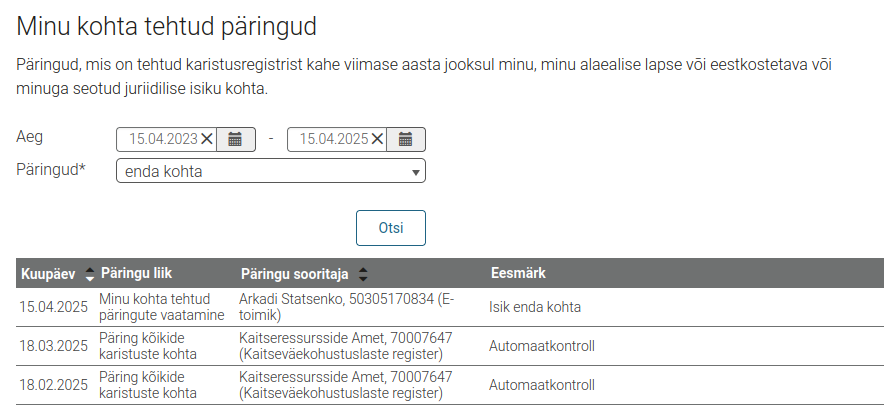
\includegraphics[width=450px]{english/figures/e-toimik.png}
\caption{E-File System (E-toimik) web interface showing data access requests. This system operates independently of the \textit{Andmejälgija} protocol and provides its own tracking mechanism for data access events \cite{e-toimik-screenshot}.}
\label{fig:e-toimik}
\end{figure}

An interesting observation regarding E-File is that similarly to the Data Tracker, it is not guaranteed to include all information about data access.

To be more specific, I once had to request a criminal record extract from Finland for employment purposes, as I had to undergo a background check. At some point I enquired about the status of my application and they responded, mentioning that it took longer than anticipated due to them also having requested my criminal record extract from Estonia, a country of my citizenship.

The inquiry to Finnish Legal Register was made on the 14th of May, 2025. Despite that there are no relevant records in the e-File system in the period from 14.05.2025 to 20.05.2025 (The day the extract was posted).

\begin{figure}[H]
\centering
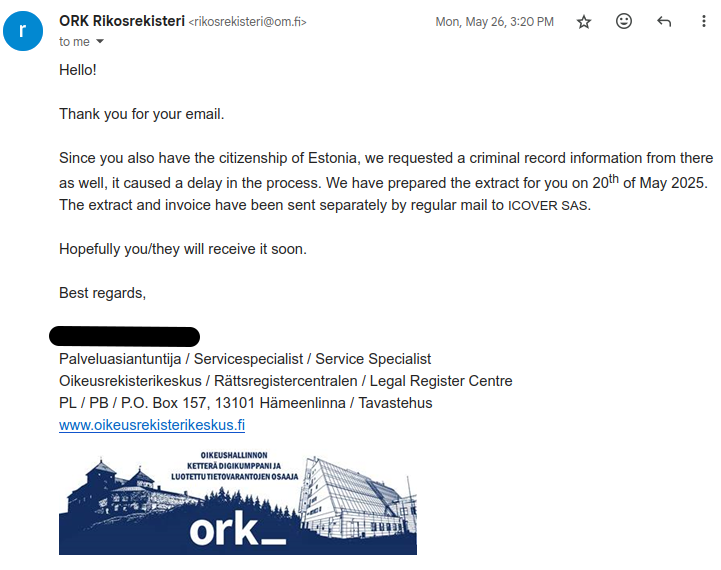
\includegraphics[width=450px]{english/figures/Screenshot from 2025-08-09 11-59-33.png}
\caption{Email response from Finnish Legal Registry confirming that they requested criminal record information from Estonia, demonstrating how data access events may not be logged in Estonian systems when authorities provide information to foreign institutions \cite{e-toimik-screenshot}.}
\label{fig:finnish-legal-registry-email}
\end{figure}

\begin{small}
\begin{center}
\begin{tabular}{|p{2.5cm}|p{4.5cm}|p{4cm}|p{2.5cm}|}
\hline
\textbf{Date} & \textbf{Query Type} & \textbf{Query Performer} & \textbf{Purpose} \\
\hline
20.05.2025 & Query for all convictions (incl. archive data) & Arkadi Statsenko (E-File) & Person about themselves \\
\hline
18.05.2025 & Query for all convictions & Defence Resources Agency, 70007647 (Conscripts Register) & Automatic control \\
\hline
15.05.2025 & Query for all convictions (incl. archive data) & Arkadi Statsenko (E-File) & Person about themselves \\
\hline
15.05.2025 & Query for all convictions (incl. archive data) & Arkadi Statsenko (E-File) & Person about themselves \\
\hline
15.05.2025 & Query for all convictions (incl. archive data) & Arkadi Statsenko (E-File) & Person about themselves \\
\hline
\end{tabular}
\end{center}
\end{small}

As shown in the table above, there is no record of Estonian authorities providing criminal record information to the Finnish Legal Registry during the period from May 14th to May 20th, 2025, despite confirmation from Finland that such a request was made. This demonstrates a significant gap in data access logging when Estonian institutions provide information to foreign authorities, highlighting limitations in the current tracking systems.


\subsection{Databases not providing any kind of data access tracking}
\begin{itemize}
    \item Schengen Information System
    \item Border Control Database (\textit{Piirikontrolli andmekogu - PIKO})
    \item Vehicle Registration Database (\textit{Liiklusregister})
    \item Court Information System (\textit{Kohtute infosüsteem - KIS})
    \item Employment register (\textit{Töötamise register (TÖR)})

\end{itemize}

These are only a few examples. There are a lot more databases that don't provide any kind of data access tracking. It is in fact much easier to count those databases that do provide some kind of data tracking than those that don't. A more complete view of what state databases exist is available from the State Information System Management System (\textit{Riigi Infosüsteemi Haldussüsteem})\footnote{\url{https://www.riha.ee/Infosüsteemid}}. At the time of writing (9.08.2025) the search returns information about 1386 databases in total, including 1100 about those in use.


